\documentclass{article}
\usepackage[utf8]{inputenc}
\usepackage{graphicx}
\graphicspath{{./Figures/}}\usepackage{algorithm}
\usepackage{ amssymb }
\usepackage[noend]{algpseudocode}
\title{Report Title}
\author{Your Name here}
\date{\today}
     
\begin{document}
     
\maketitle
     
\tableofcontents
     
\section{Introduction}
     
This is the first section.
     
Lorem  ipsum  dolor  sit  amet,  consectetuer  adipiscing  
elit.   Etiam  lobortisfacilisis sem.  Nullam nec mi et 
neque pharetra sollicitudin.  Praesent imperdietmi nec ante. \cite{alur:2015:cps}
Donec ullamcorper, felis non sodales...
     
\section{Second Section}
\subsection{image}
\begin{figure}[htbp]
    \centering
    \includegraphics[width=8cm]{gg}
    \caption{test}
    \label{fig:gg}
\end{figure}
As you can see in the figure \ref{fig:gg},Lorem  ipsum  dolor  sit  amet,  consectetuer  adipiscing  
\subsection{unordered lists}
\begin{itemize}
    \item The individual entries are indicated with a black dot, a so-called bullet.
    \item The text in the entries may be of any length.
\end{itemize}
\subsection{math}
$$E=mc^2$$

Subscripts in math mode are written as $a_b$ and superscripts are written as $a^b$. These can be combined an nested to write expressions such as

$$T^{i_1 i_2 \dots i_p}_{j_1 j_2 \dots j_q} = T(x^{i_1},\dots,x^{i_p},e_{j_1},\dots,e_{j_q})$$

We write integrals using $\int$ and fractions using $\frac{a}{b}$. Limits are placed on integrals using superscripts and subscripts:

$$\int_0^1 \frac{1}{e^x} =  \frac{e-1}{e}$$

Lower case Greek letters are written as $\omega$ $\delta$ etc. while upper case Greek letters are written as $\Omega$ $\Delta$.

Mathematical operators are prefixed with a backslash as $\sin(\beta)$, $\cos(\alpha)$, $\log(x)$ etc.

\begin{equation}
E=m
\end{equation}
\subsection{tables}
\begin{center}
    \begin{tabular}{||c c c c||} 
    \hline
    Col1 & Col2 & Col2 & Col3 \\ [0.5ex] 
    \hline\hline
    1 & 6 & 87837 & 787 \\ 
    \hline
    2 & 7 & 78 & 5415 \\
    \hline
    3 & 545 & 778 & 7507 \\
    \hline
    4 & 545 & 18744 & 7560 \\
    \hline
    5 & 88 & 788 & 6344 \\ [1ex] 
    \hline
   \end{tabular}
   \end{center}
\subsection{Algorithm}
\begin{algorithm}
    \caption{Artificial Neural Network Training Algorithm, modified from (Reed, 1999)}\label{euclid}
    \begin{algorithmic}[1]
    \Procedure{Froward Propogation}{}
    \State $\alpha^{l+1}=f(z^{l+1})$
    \State $\alpha^{l+1}=f(z^{l+1})$
    \EndProcedure
    \Procedure{Calculate Loss Function}{}
    \State $\alpha^{l+1}=f(z^{l+1})$
    \EndProcedure
    \Procedure{Backpropogation}{}
    \State $calculate~partial ~derivatives~ of~ output~ layer$
    \State $\delta_l=\frac{\partial}{\partial z_i^l}\frac{1}{2} \|h_{w,b}(x)-y\|^2=-(y_i-a_i^l)f'(z_i^l)$
    \State $calculate ~partial~ derivatives~ of~ hidden~ layers~and~update~weights$
    \State $for ~j=l-1;j>=2;j--$
    \State $\delta_l=\frac{\partial}{\partial z_i^l}\frac{1}{2} \|h_{w,b}(x)-y\|^2=-(y_i-a_i^l)f'(z_i^l)$
    \State $\delta_l=\frac{\partial}{\partial z_i^l}\frac{1}{2} \|h_{w,b}(x)-y\|^2=-(y_i-a_i^l)f'(z_i^l)p $
    \State $\delta_l=\frac{\partial}{\partial z_i^l}\frac{1}{2} \|h_{w,b}(x)-y\|^2=-(y_i-a_i^l)f'(z_i^l)$
    \State $end ~for$
    \EndProcedure
    \end{algorithmic}
    \end{algorithm}
\subsection{Minipage}
\begin{minipage}{.5\textwidth}
        \includegraphics[width=4cm]{gg}
        \label{fig:gg}
  \end{minipage}% This must go next to `\end{minipage}`
  \begin{minipage}{.5\textwidth}
        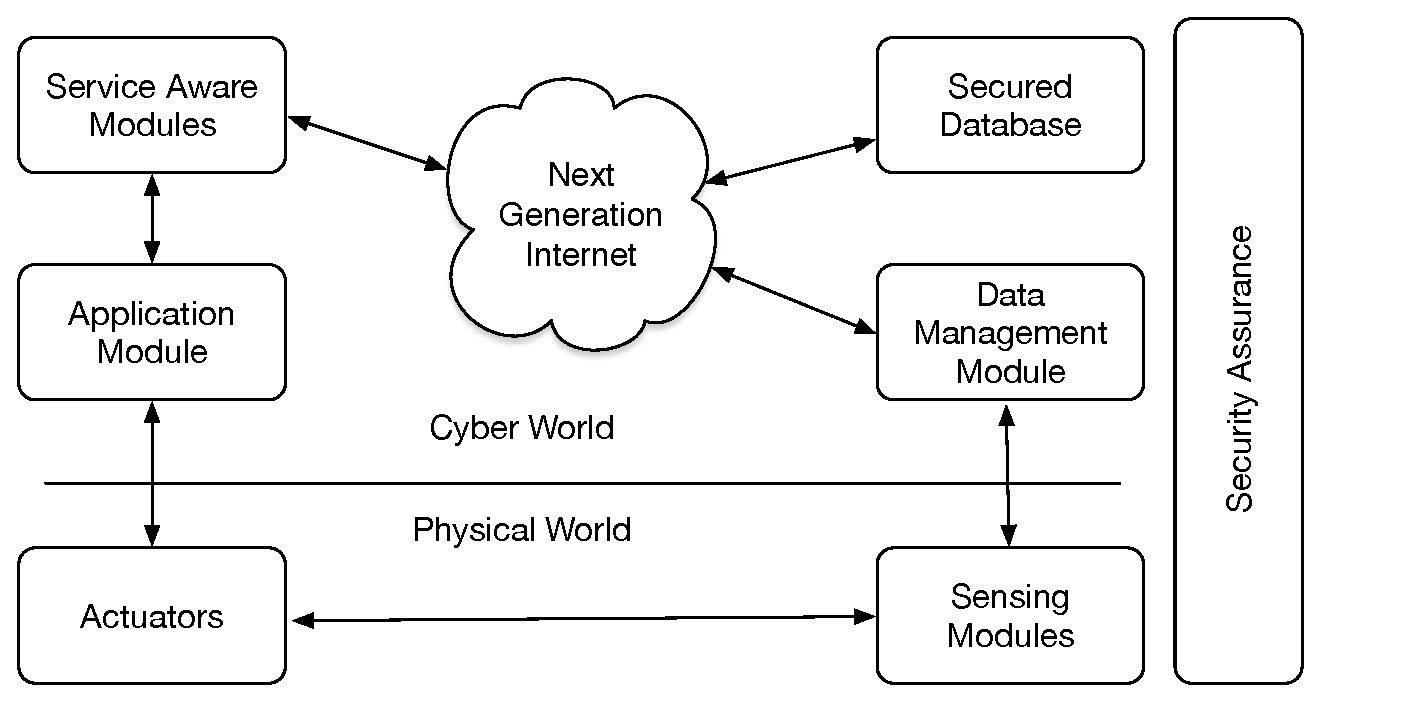
\includegraphics[width=8cm]{cps}
        \label{fig:svg}
  \end{minipage}
\subsection{useful links}
Detect hand writing math symbols\\
http://detexify.kirelabs.org/classify.html\\
create latex tables online\\
https://www.tablesgenerator.com

\bibliographystyle{apalike}
\bibliography{ref}
     
\end{document}